\chapter{物体由什么做成}\label{ch:g1:materials-around-us}

看一看早餐桌。桌上有一把勺子、一杯牛奶、一把叉子、
一张餐巾、一只碗，还有一件挂在椅背上的毛衣。
这里有许多物体，每一个都是由某种材料做成的：勺子是木头做的，叉子是金属做的，
玻璃杯是玻璃做的，餐巾是纸做的，碗是塑料做的，毛衣是羊毛做的。
一张桌子上摆满了物体，却只用了几种不同的材料。
本章就来讲这些材料。

\begin{omfigure}
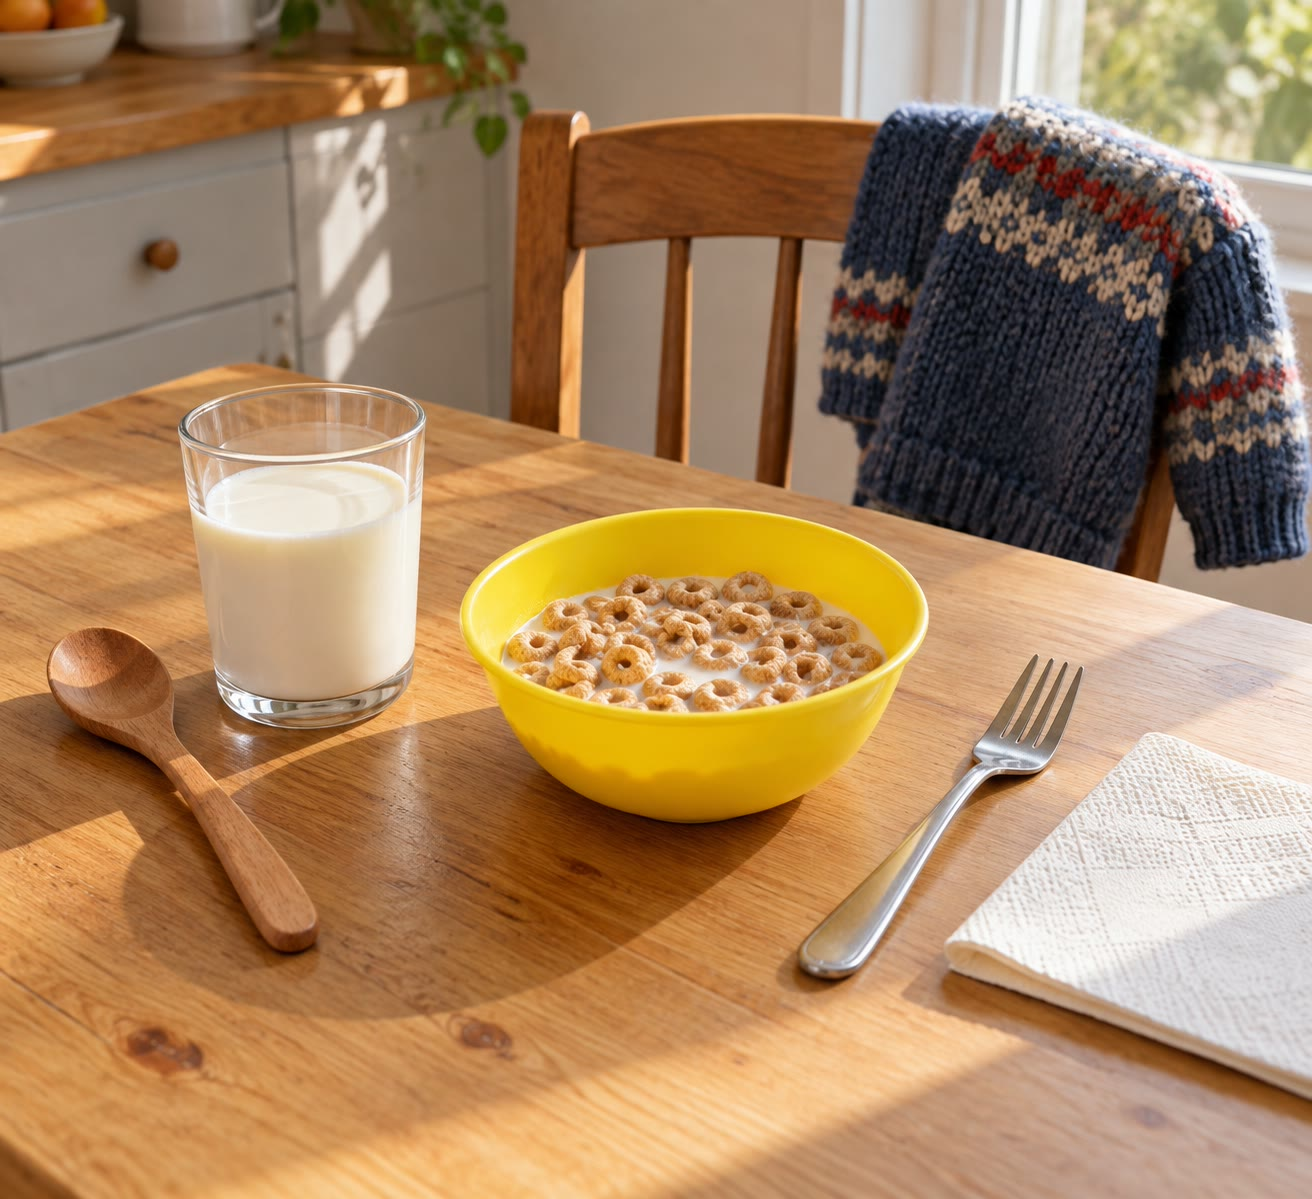
\includegraphics[width=0.62\linewidth]{images/book1/ai/g1-breakfast-table.jpg}

{\small 一张早餐桌：许多物体，由几种材料做成。}
\end{omfigure}

\section{物体与材料}

\begin{definition}[物体]\label{def:g1:materials-around-us:object}
\emph{物体}\index{物体}是指我们能看见、摸到，
并且常常拿在手里使用的东西，例如勺子、椅子、球、窗户和鞋子。
\end{definition}

\begin{definition}[材料]\label{def:g1:materials-around-us:material}
物体的\emph{材料}\index{材料}，就是物体是由什么做成的。
勺子可以用木头、金属或塑料做成：勺子是物体，
木头则是材料。
\end{definition}

\begin{example}[同一种物体，三种材料]\label{ex:g1:materials-around-us:spoons}
三把勺子并排放着。它们形状相同，用途也相同，
所以是同一类物体。但其中一把是木头做的，一把是金属做的，
还有一把是塑料做的：三种不同的材料。
\end{example}

\begin{omfigure}
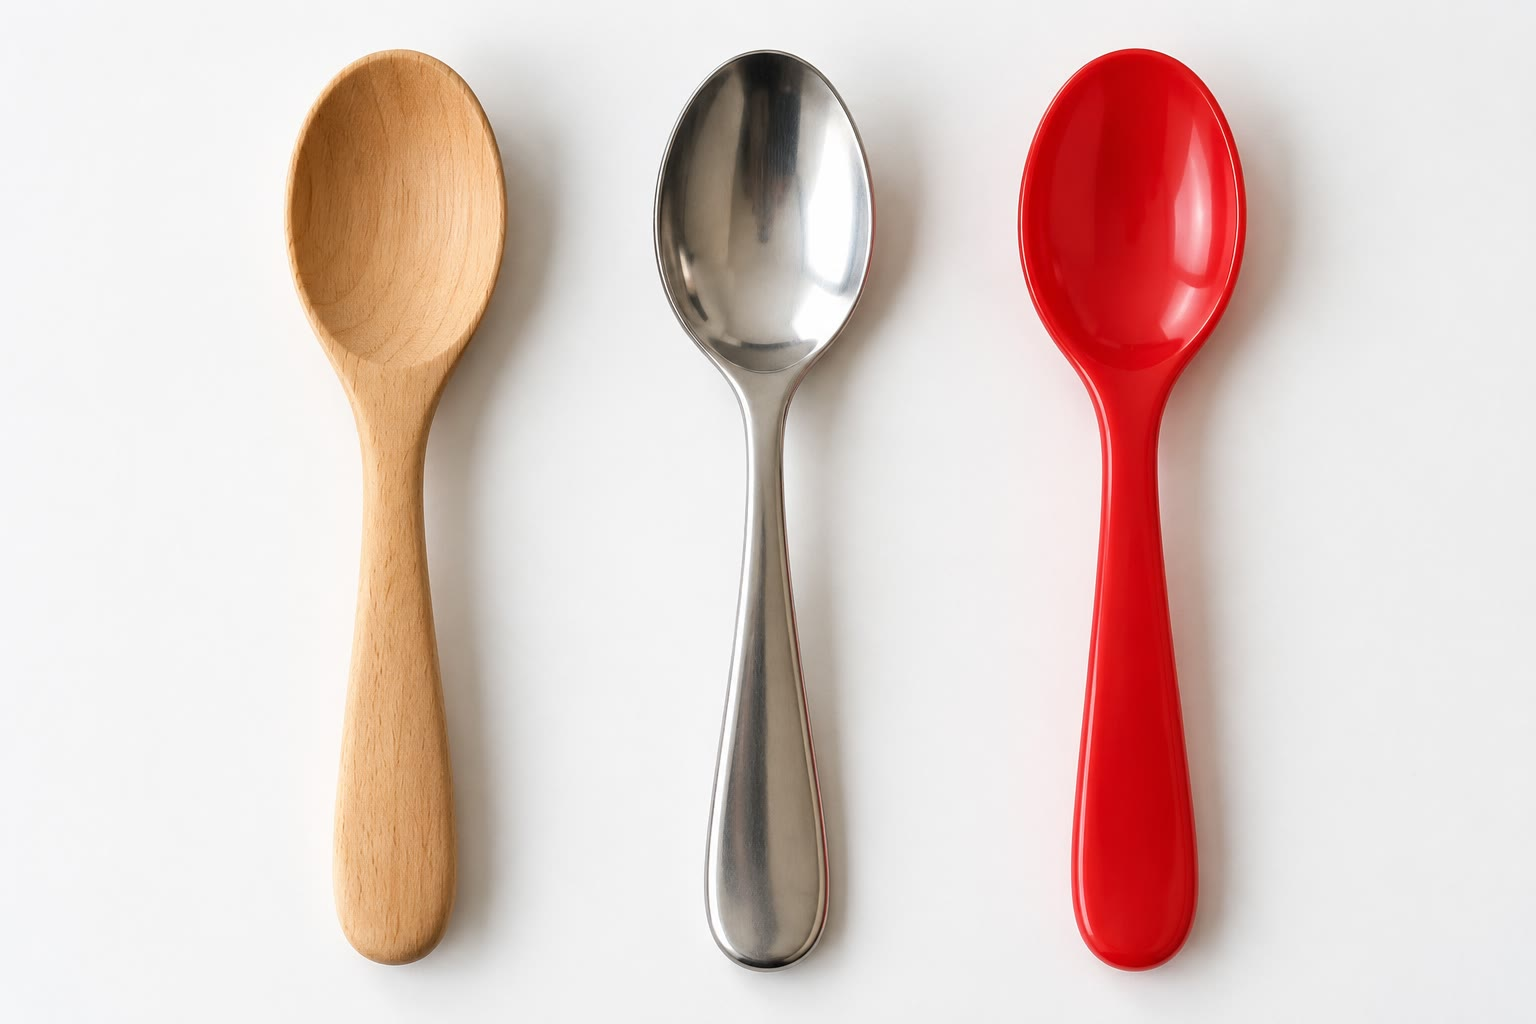
\includegraphics[width=0.55\linewidth]{images/book1/ai/g1-three-spoons.jpg}

{\small 三把勺子：同一种物体，三种材料——木头、金属
和塑料。}
\end{omfigure}

\begin{example}[同一种材料，多种物体]\label{ex:g1:materials-around-us:wood}
木头可以用来做铅笔、椅子、门、玩具火车和
木勺子。许多不同的物体可以由同一种材料做成。
\end{example}

\begin{remark}[由几种材料做成的物体]\label{rem:g1:materials-around-us:several}
许多物体由不止一种材料做成。一把剪刀
的刀片是金属的，手柄是塑料的。铅笔外面是木头，
里面是灰色的石墨芯。窗户是玻璃，嵌在
木头、金属或塑料做的窗框里。
\end{remark}

\section{常见的七种材料}

\begin{proposition}[身边的材料]\label{prop:g1:materials-around-us:seven}
我们周围的大多数物体，都是由几种常见材料做成的：
\begin{itemize}
  \item \textbf{木头}：桌子、椅子、铅笔、门；
  \item \textbf{金属}：叉子、钥匙、钉子、平底锅、自行车；
  \item \textbf{玻璃}：窗户、罐子、瓶子、玻璃杯；
  \item \textbf{塑料}：碗、瓶子、玩具、水桶；
  \item \textbf{纸和硬纸板}：书、餐巾、盒子；
  \item \textbf{织物}：衣服、窗帘、袋子——由羊毛、
        棉或其他纱线制成；
  \item \textbf{石头}：墙、台阶、鹅卵石、雕像。
\end{itemize}
\end{proposition}

\begin{omfigure}
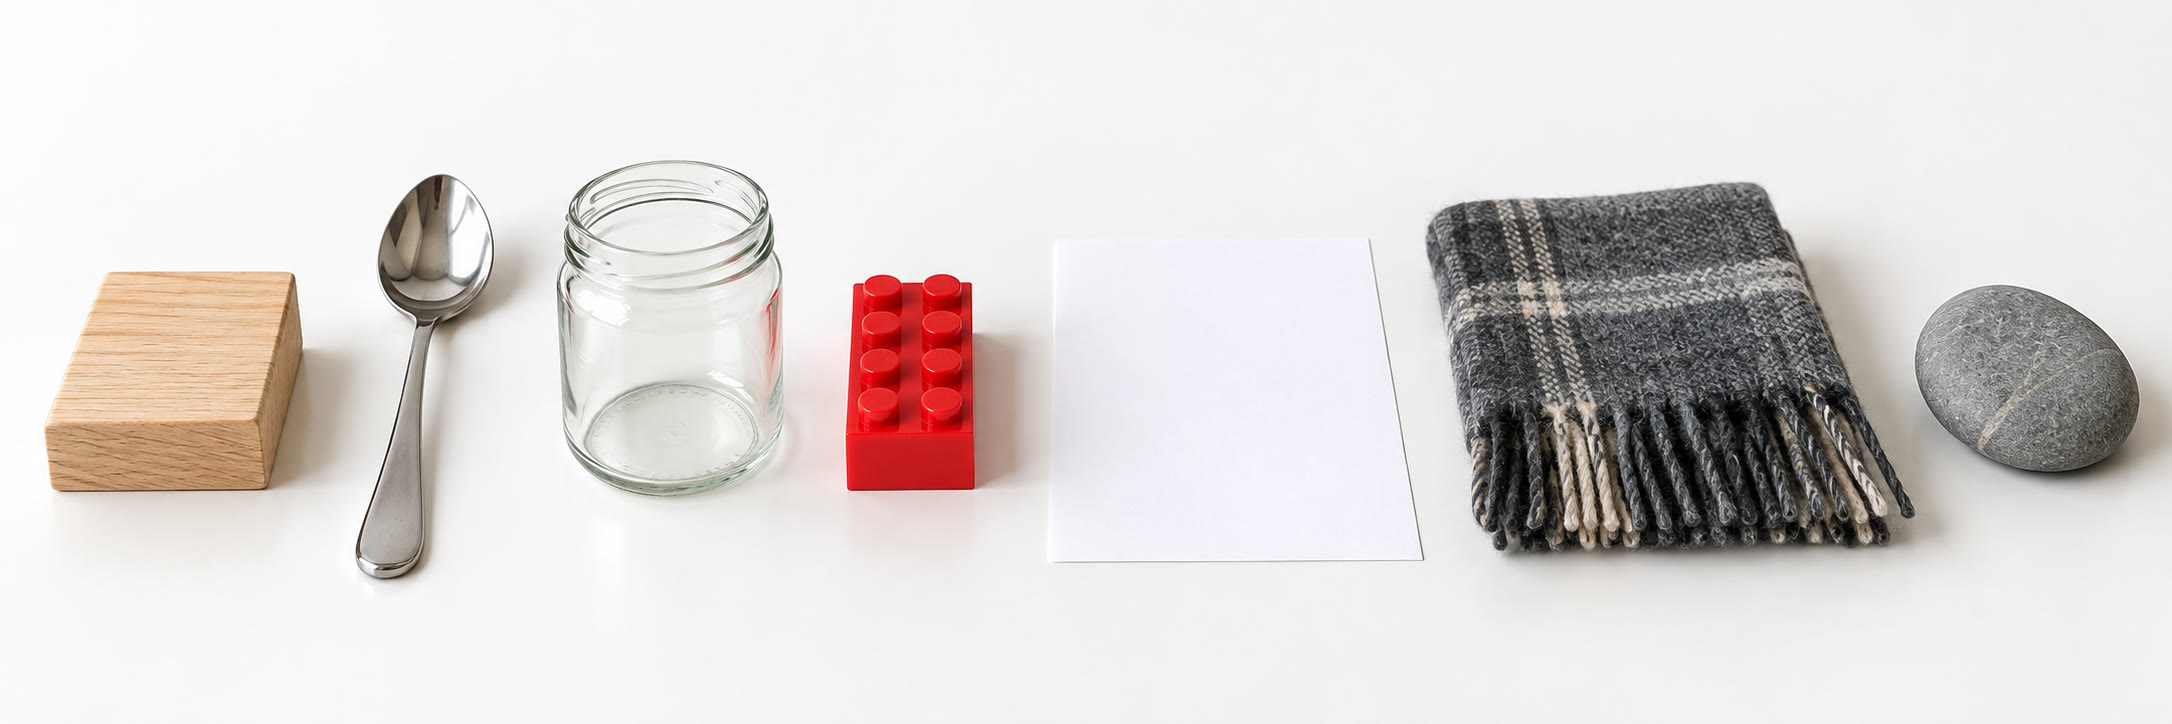
\includegraphics[width=0.75\linewidth]{images/book1/ai/g1-material-samples.jpg}

{\small 七个样品，从左到右依次为：木头、金属、玻璃、塑料、
纸、织物（羊毛）和石头。}
\end{omfigure}

\begin{remark}[与材料同名的词]\label{rem:g1:materials-around-us:names}
我们把喝水用的杯子叫作“玻璃”，因为它是由玻璃做成的，也把
一张纸叫作“纸”。这样，表示物体的词与表示材料的词
就相同了。谈论材料时，我们指的是物质本身，
而不是物体。
\end{remark}

\section{材料的性质}

\begin{definition}[材料的性质]\label{def:g1:materials-around-us:property}
\emph{材料的性质}\index{材料的性质}是指我们通过观察、
触摸或测试能够了解到的东西：它是硬的还是软的？
能不能透过它看见东西？磁铁能不能吸引它？它放在水上会不会
漂浮，还是下沉？
\end{definition}

\begin{example}[软与硬]\label{ex:g1:materials-around-us:hard}
鹅卵石是硬的：用拇指压它，不会留下痕迹。羊毛围巾
是软的：它在手里能弯曲、折叠。木头、金属、玻璃和石头
都是硬的；织物和纸是软的，很容易弯曲。
\end{example}

\begin{example}[能否透过看见]\label{ex:g1:materials-around-us:see-through}
我们可以透过窗户看到花园：玻璃能让光透过，
我们说它是\emph{透明的}。我们看不透木门、
砖墙或金属平底锅。有些塑料是透明的，像水瓶一样；
另一些则不透明，像红色的玩具积木。
\end{example}

\begin{example}[被磁铁吸引]\label{ex:g1:materials-around-us:magnet}
磁铁会把钢制回形针、钢钉或铁钥匙吸向
自己。它不会吸引木头、玻璃、塑料、纸、织物或石头。而且，
令人意外的是，它并不会吸引所有金属：铝制饮料罐和
铜丝都留在原处。磁铁吸引的是由铁和钢做成的
物体，而钢主要是铁。
\end{example}

\begin{omfigure}
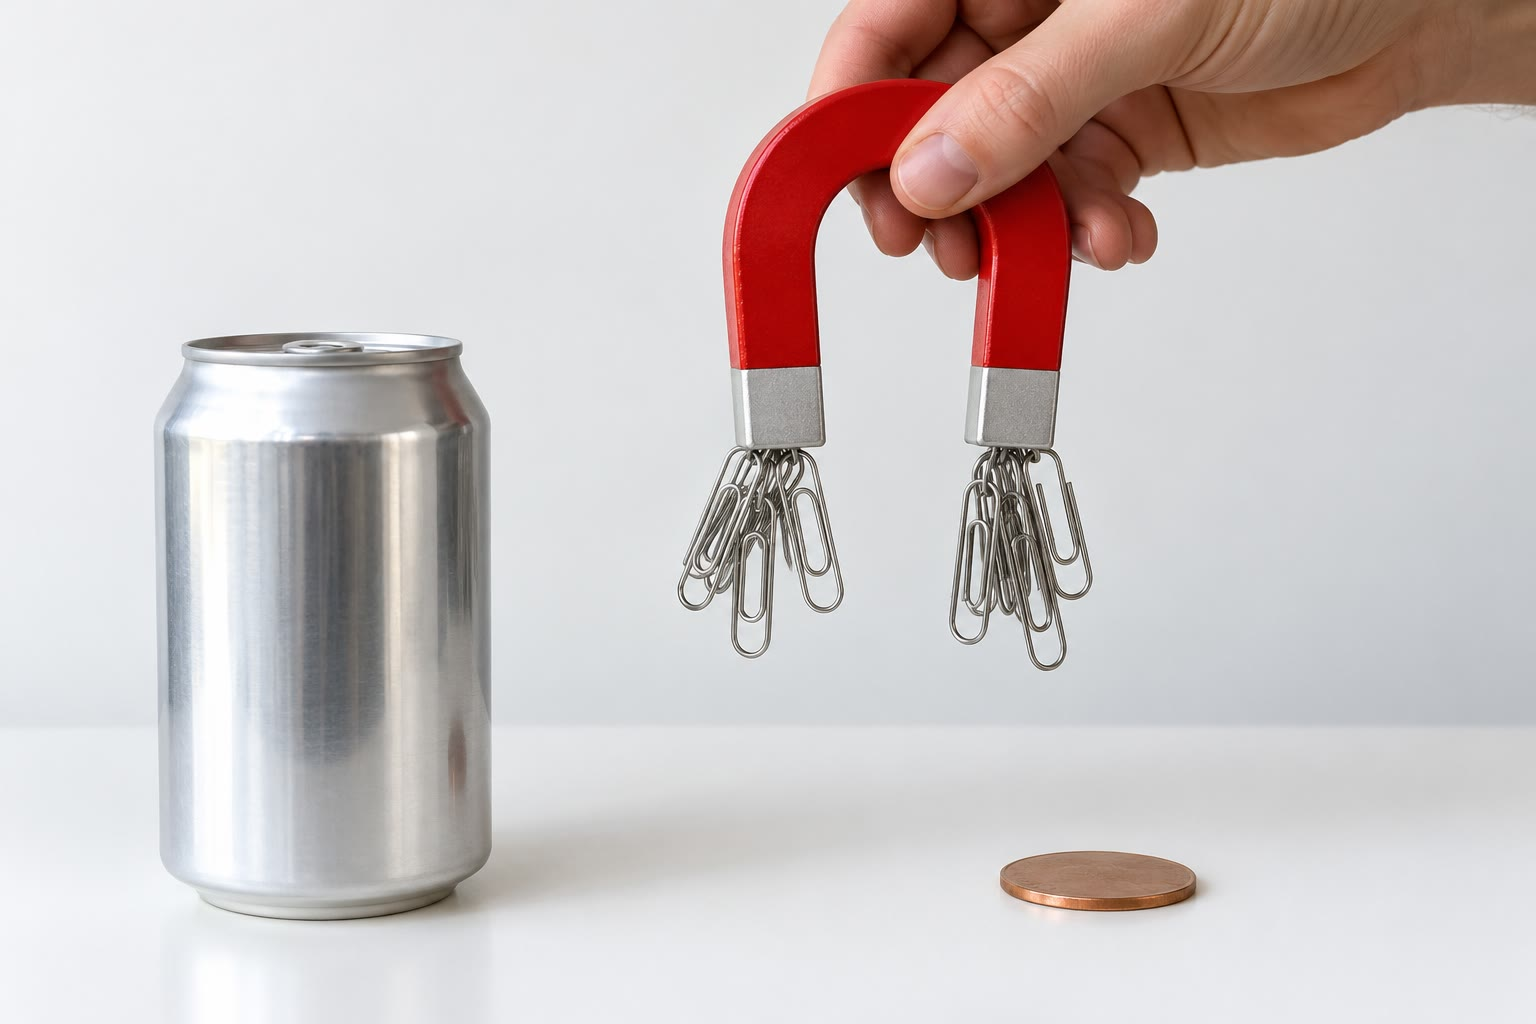
\includegraphics[width=0.55\linewidth]{images/book1/ai/g1-magnet-clips.jpg}

{\small 磁铁能吸起钢制回形针。桌上的铝制罐和
铜片都留在原处。}
\end{omfigure}

\begin{example}[漂浮与下沉]\label{ex:g1:materials-around-us:float}
在一盆水里放入几件物体。木块和塑料
瓶盖会漂浮。鹅卵石、玻璃弹珠和钢钉会沉到
盆底。物体是漂浮还是下沉，也是它
材料的性质。
\end{example}

\begin{omfigure}
\begin{tikzpicture}[font=\small]
  % the basin
  \fill[omWater!80] (0,0) rectangle (9,2.2);
  \draw[omGlass, line width=0.8pt] (-0.1,2.7) -- (0,2.6) -- (0,0) -- (9,0)
    -- (9,2.6) -- (9.1,2.7);
  % floating: wooden block, plastic cap
  \fill[brown!55, draw=brown!70!black] (0.8,2.0) rectangle (2.2,2.5);
  \fill[red!70, draw=red!50!black] (3.7,2.05) rectangle (4.3,2.35);
  % sunk: pebble, marble, nail
  \fill[black!35, draw=black!60] (5.0,0.25) ellipse (0.45 and 0.22);
  \shade[ball color=cyan!40] (6.5,0.2) circle (0.18);
  \fill[black!55] (7.6,0.06) rectangle (8.6,0.14);
  \fill[black!55] (7.52,0.02) rectangle (7.62,0.18);
  % labels
  \node[anchor=south] at (1.5,2.75) {木块};
  \node[anchor=south] at (4.0,2.75) {塑料瓶盖};
  \node[anchor=north] at (5.0,-0.1) {鹅卵石};
  \node[anchor=north] at (6.5,-0.1) {玻璃弹珠};
  \node[anchor=north] at (8.1,-0.1) {钢钉};
  \node[anchor=west, align=left] at (9.3,2.2) {会漂浮};
  \node[anchor=west, align=left] at (9.3,0.2) {会下沉};
\end{tikzpicture}

{\small 盆中水里：木块和塑料瓶盖漂浮；
鹅卵石、玻璃弹珠和钢钉下沉。}
\end{omfigure}

\section{材料的分类}

\begin{method}[按一种性质分类]\label{met:g1:materials-around-us:sort}
对一堆物体进行分类：
\begin{enumerate}
  \item 选择\textbf{一个}问题，例如
        “磁铁会吸住它吗？”；
  \item 逐一检验每件物体，并把它放入“能”组
        或“不能”组；
  \item 如需要，可再用另一个问题把每组重新分类。
\end{enumerate}
每次只用一个问题：这样，每件物体都恰好有一个位置。
\end{method}

\begin{omfigure}
\begin{tikzpicture}[font=\small]
  \draw[omDef, line width=1pt] (0,0) circle (2.3);
  \draw[omProp, line width=1pt] (2.4,0) circle (2.3);
  \node[omDef, font=\small\bfseries] at (-0.6,2.65) {由金属制成};
  \node[omProp, font=\small\bfseries] at (3.0,2.65) {被磁铁吸引};
  \node[font=\footnotesize] at (-1.1,0.35) {饮料罐};
  \node[font=\footnotesize] at (-1.1,-0.35) {铜丝};
  \node[font=\footnotesize] at (1.2,0.6) {钢钉};
  \node[font=\footnotesize] at (1.2,0) {铁钥匙};
  \node[font=\footnotesize] at (1.2,-0.6) {回形针};
  \node[font=\footnotesize] at (3.5,0) {（无）};
  \node[anchor=west] at (5.2,0.9) {木勺};
  \node[anchor=west] at (5.2,0.3) {玻璃弹珠};
  \node[anchor=west] at (5.2,-0.3) {羊毛围巾};
  \node[anchor=west] at (5.2,-0.9) {鹅卵石};
\end{tikzpicture}

{\small 两个问题，两个圈。蓝圈内：由金属
制成的物体。橙圈内：能被磁铁吸引的物体。
两圈重叠处：铁或钢制成的物体。两圈之外：其余一切。}
\end{omfigure}

\begin{center}
\small
\begin{tabular}{lccc}
\hline
物体（材料） & 是否坚硬？ & 是否透明？ & 能否被磁铁吸引？ \\
\hline
木块（木材） & 是 & 否 & 否 \\
钢钉（钢） & 是 & 否 & 是 \\
玻璃弹珠（玻璃） & 是 & 是 & 否 \\
瓶盖（塑料） & 是 & 否 & 否 \\
纸片（纸） & 否 & 否 & 否 \\
围巾（羊毛） & 否 & 否 & 否 \\
鹅卵石（石头） & 是 & 否 & 否 \\
\hline
\end{tabular}
\end{center}

\section{为用途选择合适的材料}

\begin{proposition}[每种材料都根据其性质来选择]\label{prop:g1:materials-around-us:choose}
人们根据物体必须完成的任务来选择它的材料：
\begin{itemize}
  \item 窗户必须让光透进来：它由玻璃制成，玻璃
        是透明的；
  \item 雨衣必须挡住雨水并且能够折叠：它由
        塑料或水无法透过的织物制成；
  \item 锅在炉灶上不能熔化：它由金属制成；
  \item 锅柄不能烫手：它常由木头
        或硬塑料制成，这两者不会像金属那样烫手；
  \item 枕头必须柔软：它由填充了羽毛
        或纤维的织物制成。
\end{itemize}
\end{proposition}

\begin{example}[小船]\label{ex:g1:materials-around-us:boat}
一艘玩具船必须能够漂浮。它可以用木头或塑料制成。
用一块实心石头做成的小船会立刻下沉。
\end{example}

\begin{remark}[打碎的玻璃]\label{rem:g1:materials-around-us:glass}
玻璃很硬，但会碎裂，碎片很锋利。当一块玻璃
破碎时，大人会把碎片捡起来。
\end{remark}

\section{练习}

\begin{exercise}[$\star$]\label{exo:g1:materials-around-us:1}
椅子是物体还是材料？木头是物体还是材料？
\end{exercise}

\begin{exercise}[$\star$]\label{exo:g1:materials-around-us:2}
说出每件物体的材料：窗玻璃、钉子、鹅卵石、
书、袜子。
\end{exercise}

\begin{exercise}[$\star$]\label{exo:g1:materials-around-us:3}
举出两件木制物体和两件塑料制物体。
\end{exercise}

\begin{exercise}[$\star$]\label{exo:g1:materials-around-us:4}
找出不同类的一件，并说明理由：木勺、金属叉、
塑料勺、木椅。（看看材料。）
\end{exercise}

\begin{exercise}[$\star$]\label{exo:g1:materials-around-us:5}
我们能透过哪种材料看到另一侧：木头、玻璃还是石头？
\end{exercise}

\begin{exercise}[$\star$]\label{exo:g1:materials-around-us:6}
把一块磁铁靠近一枚钢钉、一颗玻璃弹珠和一块木块。
它会吸引哪一个？
\end{exercise}

\begin{exercise}[$\star$]\label{exo:g1:materials-around-us:7}
看看带水盆的图。有几件物体漂浮？有几件
下沉？
\end{exercise}

\begin{exercise}[$\star$]\label{exo:g1:materials-around-us:8}
一把剪刀有刀片和把手。每个部分由哪种
材料制成？一把剪刀是由一种材料还是两种材料制成的？
\end{exercise}

\begin{exercise}[$\star$]\label{exo:g1:materials-around-us:9}
看看带两个圈的图。饮料罐在哪个圈里？
为什么它不在橙色的圈里？
\end{exercise}

\begin{exercise}[$\star\star$]\label{exo:g1:materials-around-us:10}
窗户为什么用玻璃做，而不用木头做？
\end{exercise}

\begin{exercise}[$\star\star$]\label{exo:g1:materials-around-us:11}
萨姆想用“磁铁能否吸引它？”这个问题给这8件物体分类：
一枚钢钉、一个回形针、一块鹅卵石、一把木勺、一把铁钥匙、
一个饮料罐、一颗玻璃弹珠、一只羊毛袜。有多少件物体应放入
“是”组？有多少件放入“否”组？
\end{exercise}
